\subsubsection{Backgrounds from particle misidentification}
\label{sec:backgrounds:misid}

A possible source of contamination comes from particles which are incorrectly identified as the
$\Kstarz\mumu$ final state.  A meson that decays \decay{X}{hh^\prime} which is then reconstructed under the incorrect mass
hypothesis could pass the selection criteria.
This type of contamination is studied by assigning different mass hypotheses to each final state
particle and calculating the invariant mass of the \mumu and \kpi candidates.
If the mass of one of these objects is seen to peak at the mass of a known particle, then the
contamination is removed  by applying particle identification (PID) criteria to particles whose reassigned invariant mass falls near $m(X)$.

Since PID and mass criteria have already been applied, little background is expected to
contaminate the \Kstarz  candidate.
The following combinations of masses are checked.
The notation $m(AB\leftrightarrow CD)$ denotes the invariant mass of $AB$ under the mass hypotheses of $CD$.
\begin{itemize}
  \item A real \pipi identified as \kpi.
    Contamination from either the decay \decay{\KS}{\pipi} or \decay{\rho}{\pipi} is not seen.
  \item A real \kk identified as \kpi.
    There is a small contribution from the decay \decay{\phi}{\kk} observed.
    To remove this contribution all candidates whose mass is within 10\mev of the $\phi$ mass under
    the \kk hypothesis
    are rejected if they also satisfy {\tt ProbNNpi$(\pi)>0.3$} and {\tt ProbNNK$(\pi)<0.3$}.
  \item A real \mumu identified as \kpi.
    The largest source of real dimuon background would be from the decays \decay{\phi}{\mumu},
    \decay{\jpsi}{\mumu} and \decay{\psitwos}{\mumu}.
    However, the mass constraint on the \kpi system results in a
    distribution of $m(\kpi\leftrightarrow\mumu)<850\mev$, significantly less than the $\phi$,
    \jpsi and \psitwos resonances.
    There is no need to remove anything from this mass swap.
\end{itemize}
Potential backgrounds from double misidentification of the \mumu pair from the most common hadronic
states are also considered.
\begin{itemize}
  \item A real \kpi identified as a \mumu.
    The \Dz has a finite lifetime, and its most common decay is to the $\Kp\pim$ final state.
    A small peak in $m(\Kp\pim)$ is observed at the \Dz mass, which is removed
    by rejecting candidates with
    {\tt ProbNNmu$(\mu)<0.3$} and the \mumu mass is within $25\mev$ of $m(\Dz)$ under the \kpi hypothesis.
  \item A real $\pipi$ identified as $\mumu$.
    Events forming a mass $m(\mumu\leftrightarrow\pipi)$ within $25\mev$ of the known \KS mass are
    vetoed.
    %Here, the decay \decay{\KS}{\pipi} is observed.
    %The candidate is removed if either muon has {\tt ProbNNmu$<0.3$} and the \pipi mass
    %is within $25\mev$ of $m(\KS)$.
  \item A real $\Lambda^0\!\to\proton\pim$ identified as $\mumu$.
     After applying stringent PID constraints a potential \Lz contamination is seen.  This is removed by requiring that {\tt ProbNNp$(\mu)<0.3$} for candidates within $10\mev$ of the \Lz
    mass.
  \item A real \kk identified as a \mumu.  No evidence of \decay{\phi}{\kk} is seen, where both kaons are misidentified as
    muons.
    There is, however, a potential background source at $m(\mumu\leftrightarrow\kk)=1070\mev$, this
    is discussed in \Sec{sec:x1070}.
    %requiring $|m(\mumu\leftrightarrow\Kp\Km)-m(\phi)|>10$ and
    %$|m(\mumu\leftrightarrow\Kp\Km)-m(X(1070))|>10\mev$
    %The $X(1070)$ is a very poorly known state, but has a mass of $1072\pm1\mev$ and a width of
    %$3.5 \pm0.57$, which is consistent with our observations.
    %This was challenging to remove completely using PID vetoes, and therefore, if the new $\Kp\Km$
    %mass is within $10\mev$ of $1072\mev$, then the candidate is vetoed.
\end{itemize}
Appendix~\ref{app:misid} contains plots showing the effect of these PID swaps and vetoes.
A summary of the vetoes used to remove \Bp candidates with double misidentification are given in
Table~\ref{tab:bkg:vetoes}.
It is clearly difficult to assess these constraints using a single simulated sample, because the
requirements are based on mass swaps, for example the cut to remove the \KS is very unfavourable
towards the $500\mev$ sample.
However, applying the cuts in Table~\ref{tab:bkg:vetoes} to the SM \btokstrmumu simulated sample
show that the cuts are close to 100\% signal efficient.


\begin{table}
  \caption{\small
   Vetoes from double and single misidentification of particles.
    %If there is nothing in the PID column, then all candidates in the region are removed, otherwise
    %only those failing the PID criteria are removed.
    %If there is nothing in the PID column, then all candidates in the region are removed, otherwise
    %only those failing the PID criteria are removed.
    If, under the alternate hypothesis, the \db or \Kstarz candidate mass falls within the range
    indicated under, the candidates are subject to the PID requirements (no PID requirements
    indicate absolute vetoing).
  }
  \label{tab:bkg:vetoes}
  \begin{center}
    \begin{tabular}{lcc}\toprule
      \multicolumn{2}{c}{Mass} & PID \\\midrule
      $\left|m(\kpi\leftrightarrow\kk) - m^{PDG}_\phi\right|$ & $<10$
      & {\tt ProbNNpi$(\pi)>0.3$} and {\tt ProbNNK$(\pi)<0.3$}\\
      $\left|m(\mumu\leftrightarrow\pipi) - m^{PDG}_{\KS}\right|$ & $<25$ &  \\
      $\left|m(\mumu\leftrightarrow\kpi) - m^{PDG}_{\Dz}\right|$& $<25$ & {\tt ProbNNmu$(\mu)>0.3$} \\
      $\left|m(\mumu\leftrightarrow p\pim) - m^{PDG}_{\Lz}\right|$& $<10$
      & {\tt ProbNNp$(\mu)<0.3$}  \\\bottomrule
    \end{tabular}
  \end{center}
      %$\left|m(\mumu\leftrightarrow\kk) - m^{PDG}(\phi)\right| < 10$ & --- \\
      %$\left|m(\mumu\leftrightarrow\kk) - m^{PDG}(X(1072))\right| < 10$ & --- \\
\end{table}

There are also contributions from the decay \decay{\Bd}{\jpsi\Kstarz} and \decay{\jpsi}{\mumu},
where one of the hadron is misidentified as a muon, and vice versa.
This can be trivially removed by requiring that the hadrons do not satisfy {\tt isMuon}, as shown
in \Fig{fig:bkg:doublemisid}.

%\begin{figure}
  %\begin{center}
    %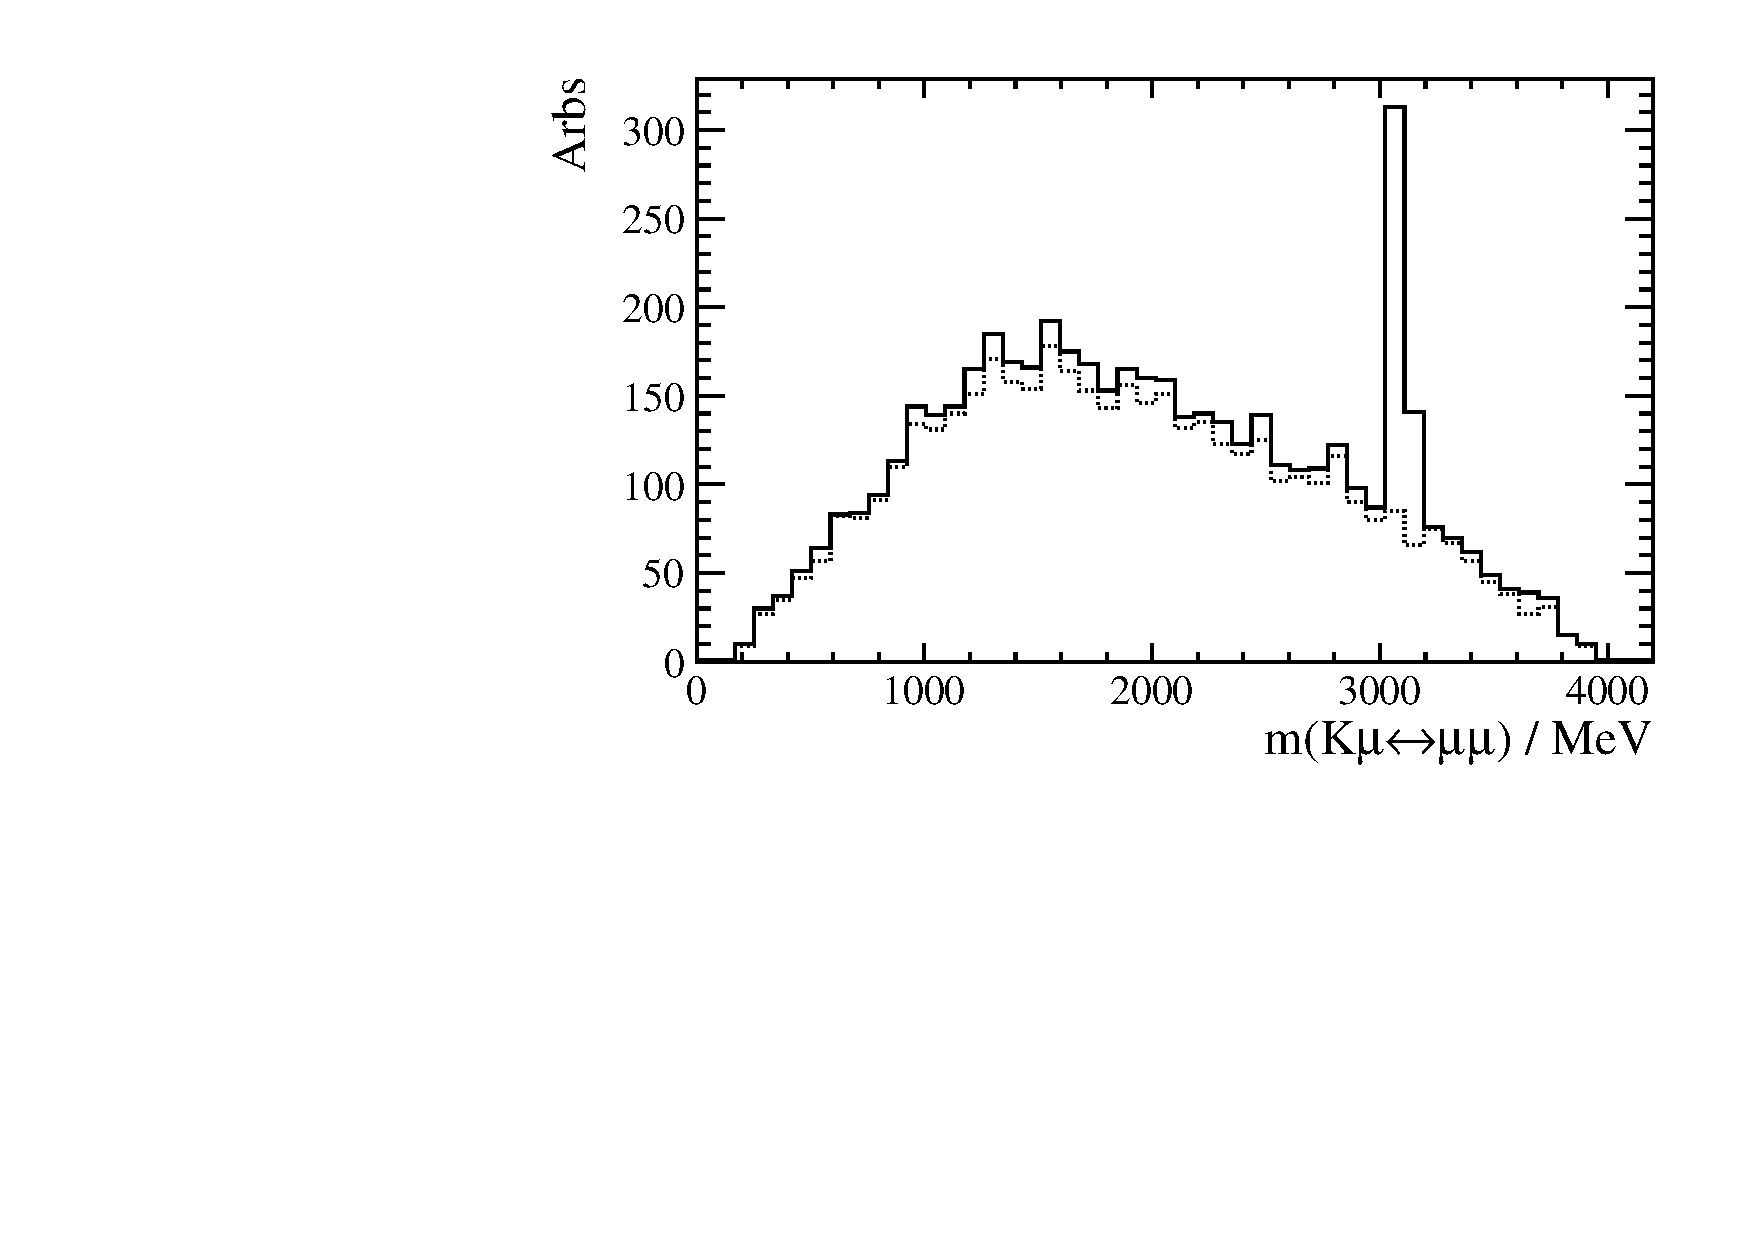
\includegraphics[width=0.48\textwidth]{double_misid_pi}
    %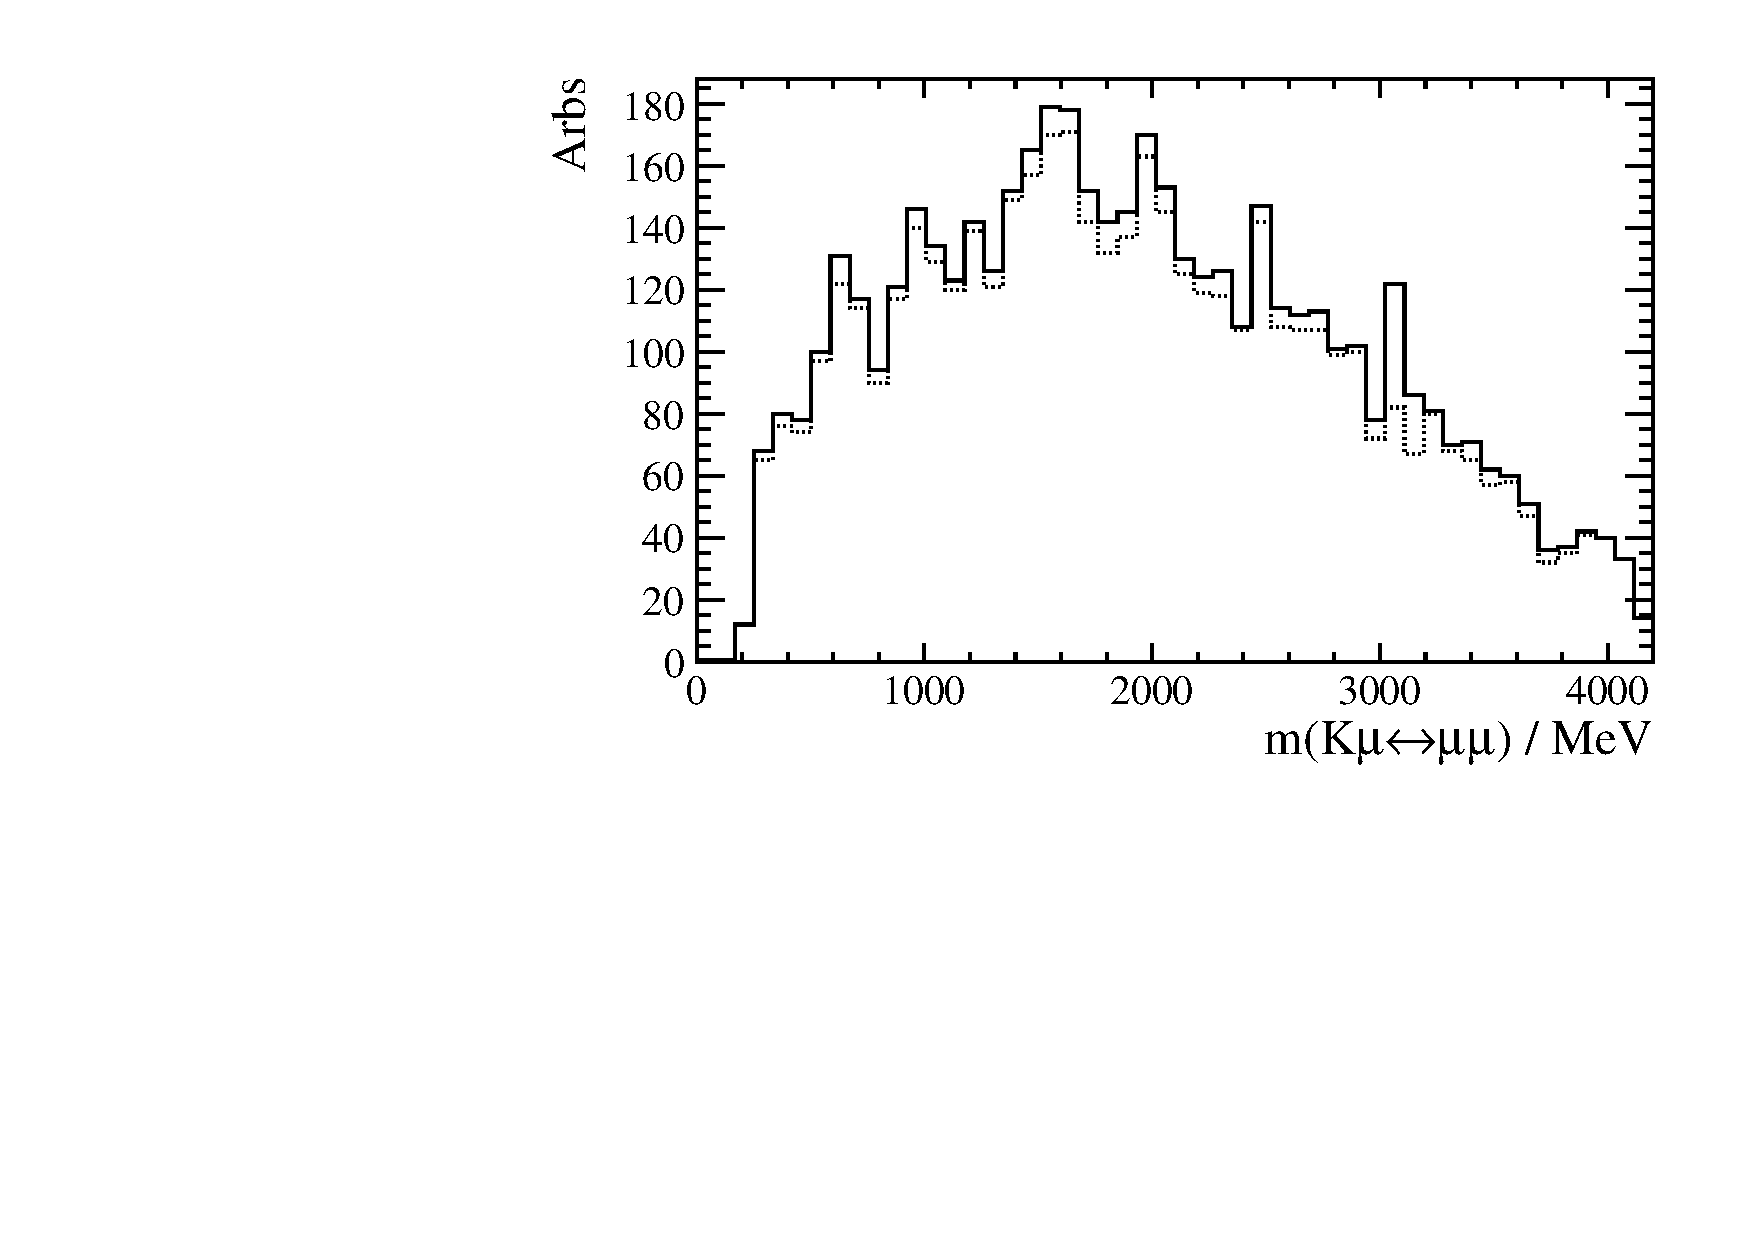
\includegraphics[width=0.48\textwidth]{double_misid_k}
    %\caption{\small
      %Background contributions from \decay{\Bd}{\jpsi\Kstarz}, where both a muon and (left) pion
      %and (right) kaon are misidentified as one another.
      %This background is very effectively removed by requiring that the hadron does not satisfy the
      %{\tt isMuon} criteria; the effect of this veto is shown with a dotted line.
    %}
    %\label{fig:bkg:doublemisid}
  %\end{center}
%\end{figure}

The sidebands are used to estimate the level of background in the signal region, and therefore
background
contributions are only problematic if they produce a narrow peaking structure in the dimuon mass.
Since misidentification results in smearing out of the mass, in general misidentification can only cause a problem if the decaying particle has roughly zero natural width.
Therefore, any remaining misidentification-type backgrounds have negligible effect in the analysis.






